\documentclass{article}
\input{../../../../LaTex/preamble/preamble_article.tex}



\begin{comment} 
    重复语句

    \vspace{0.5em}

        \item[] \textbf{(单选)检测:} (\qquad)
        
        \begin{enumerate}[label=\Alph*.]
            \item 
            \item 
            \item 
            \item 
        \end{enumerate}

        \textbf{答案:} 

        \textbf{解析:} 
        
        \hspace{2em}
   

\end{comment}


\title{高中物理讲义}

\author{学生: 谢 \quad 教师: 马祥芸}

\begin{document}

\maketitle
\tableofcontents
\newpage
\zihao{-4}

\section{半期试卷结构}
\subsection{考纲分布}
\begin{itemize}
    \item 科学常识(单选4分):

          \begin{enumerate}
              \item 亚里士多德认为物体下落的快慢与它的轻重(质量)有关,这种观念是错误的

                    \vspace{-1em}

                    \hspace{-1em}\begin{adjustbox}{minipage=0.91\linewidth, bgcolor=gray!20, padding=1em}
                        \small % 将字号变小为 small
                        亚里士多德(公元前$384\sim322$年)提出过许多错误的观点和理论,但是我们应该辩证地看待,保持尊重
                    \end{adjustbox}

                    \vspace{-1em}

              \item 伽利略通过\textbf{比萨斜塔实验},论证了自由落体的物体下落快慢与轻重(质量)无关
              \item 伽利略的\textbf{斜面滑块实验}论证了小球的匀加速运动的大小与斜面倾斜程度无关
              \item 牛顿三定律:
                    \begin{itemize}
                        \item \textbf{第一定律(惯性定律):} $ F = 0 \quad \lra \quad $物体保持静止或匀速运动
                        \item \textbf{第二定律(运动定律):} $ \va{F} = m \, \va{a} $
                        \item \textbf{第三定律(作用与反作用定律):} $ \va{F}_{AB} = - \va{F}_{BA} $ 力是成对存在的,大小相等方向相反
                    \end{itemize}
              \item 平行四边形定则: 保持匀速或静止的物体,力的合成为\textbf{零向量$\va{0}$}
              \item 托勒密地心说: 地球是宇宙的中心,是静止的,太阳和月亮以及其他星体围绕地球转
              \item 哥白尼日心说: 太阳是宇宙的中心,地球和其他行星围绕太阳转
              \item 第谷: 精确的天文数据为日后开普勒的行星运动定律的发现提供了重要的\textbf{观测依据}
              \item 开普勒行星运动定律:
                    \begin{itemize}
                        \item \textbf{第一定律(椭圆轨道定律):} 运动的轨道是椭圆,太阳位于椭圆的一个焦点上
                        \item \textbf{第二定律(面积定律):} 行星在相等时间内,在轨道上扫过的面积相等
                        \item \textbf{第三定律(调和定律):} $ \frac{a^{3}}{T^{2}} = k $ 其中$a$是轨道半长轴
                    \end{itemize}
              \item 胡克等科学家: 行星绕太阳运动是因为受到了\textbf{引力},甚至证明了与距离的二次方成反比
              \item 牛顿万有引力定律: $ \va{F} = G\dfrac{m_{1}m_{2}}{\va{r}^{2}}$
              \item 卡文迪什通过\textbf{扭秤实验}测量了万有引力常量$G = 6.67 \cross 10^{-11} \, N \vdot m^{2}/kg^{2} $

                    \vspace{-1em}

                    \hspace{-1em}\begin{adjustbox}{minipage=0.91\linewidth, bgcolor=gray!20, padding=1em}
                        \small % 将字号变小为 small
                        石英丝连接细杆,两端放置等大质量球,在两球附近放置两大质量球产生引力矩,用光线反射法放大扭转

                        \vspace{-1em}

                        $$ \theta \propto \text{力矩} \quad \lra  \quad k\theta = 2F_{G}L \quad (k\text{为比例系数需提前测量}) $$
                    \end{adjustbox}

                    \vspace{-1em}

              \item 亚当斯和勒维耶利用万有引力定律计算出了"新"行星的轨道
              \item 伽勒和勒维耶发现了这颗行星,后被命名为海王星
              \item 哈雷利用万有引力预言了同一彗星的按时回归,后被命名为"哈雷彗星"
              \item 钱学森被誉为"中国航天之父",地球同步卫星的(赤道)轨道高度$36000km$
              \item 阿姆斯特朗:人类登月第一人 \quad 杨利伟:中国登月第一人
          \end{enumerate}

          \vspace{0.5em}

    \item[] \textbf{(单选)检测:} 下列选项中符合科学历史的常识是(\qquad)

        \begin{enumerate}[label=\Alph*.]
            \item 托勒密提出了日心说否定了地心说
            \item 牛顿通过扭秤实验测量了引力常量$G$
            \item 亚当斯和勒维耶利用万有引力定律计算出了一个"新"行星的轨道
            \item 第谷测量精确的天文数据为日后哈雷彗星的周期计算提供了重要的观测数据
        \end{enumerate}

        \textbf{答案:} C

        \textbf{解析:}

        \hspace{2em}海王星的轨道计算,和星球发现均有\textbf{勒维耶}的参与;
        第谷的测量数据为开普勒的行星运动定律提供了重要的观测数据

        \newpage

    \item 运动分类(单选4分):
          \begin{itemize}
              \item 自由落体: \textbf{仅}受重力的竖直向下运动
              \item 平抛运动: 水平方向速度恒定,竖直方向自由落体,轨迹为\textbf{抛物线}(斜抛同样成立)
              \item 圆周运动: 围绕某点或轴沿着圆形轨道运动,加速度指向圆心,速度方向沿切线
              \item 曲线运动: 速度方向随时发生变化,加速度方向不定,\textbf{曲率半径}描述轨迹弯曲程度
              \item 绕星运动: 引力作用下的运动,椭圆或近似圆周轨道
          \end{itemize}

          \vspace{1em}

    \item[] \textbf{(单选)检测:} 下列对物理现象的说明正确的是(\qquad)

        \begin{enumerate}[label=\Alph*.]
            \item 运动员投出的篮球,忽略空气阻力影响,其运动轨迹是抛物线
            \item 陨石穿过大气层落到地面的过程是自由落体运动
            \item 地球围绕着太阳做严格的圆周运动
            \item 坐在匀速圆周运动的旋转木马上,加速度的大小为0
        \end{enumerate}

        \textbf{答案:} A

        \textbf{解析:}

        \hspace{2em}无阻力的斜抛运动其轨迹也是抛物线;穿过大气层时受到空气阻力,非自由落体;
        地球围绕太阳运动的轨道是椭圆近似圆周;匀速圆周运动仍有加速度指向圆心

        \vspace{2em}

    \item 机械能守恒现象(单选4分):

          \hspace{2em}主要考察物体机械能的概念:\textbf{动能$E_{k}$}与\textbf{重力势能$E_{g}$},方法归纳:
          \begin{itemize}
              \item 有无摩擦力
              \item 有无弹簧的弹性势能变化
              \item 有无其他外力做功
              \item 碰撞,绳子突然绷紧通常不守恒
              \item \textbf{整个过程仅有动能与重力势能之间的能量转化}
          \end{itemize}

          \vspace{1em}

    \item[] \textbf{(单选)检测:} (\qquad)

        \begin{enumerate}[label=\Alph*.]
            \item 从滑梯上匀速滑下的小朋友机械能守恒
            \item 被踢出的足球,离开脚面后在空中的运动(忽略空气阻力)过程中足球机械能守恒
            \item 光滑平面上运动的物体碰撞另一物体后粘连运动,两者组成的系统机械能守恒
            \item 自由落体的物体下落压缩一弹簧并向上弹的过程机械能守恒一直守恒
        \end{enumerate}

        \textbf{答案:} B

        \textbf{解析:} 滑梯有摩擦力;碰撞没有特别说明通常机械能不守恒;
        考虑始末状态机械能守恒,但非一直保持机械能守恒,弹簧具有弹性势能

        \hspace{2em}

    \item 万有引力

          空着    \\
          空着    \\
          空着    \\

          \hspace{2em}

    \item 功能关系
          \begin{enumerate}
              \item[一、] 功(Work)
                  \begin{enumerate}
                      \item 定义:力在物体位移的方向上产生作用(标量)$ W = \va{F} \vdot \va{x} = Fx\cos{\theta}$,单位\textbf{焦耳$J$}

                            \vspace{-1em}

                            \hspace{-1em}\begin{adjustbox}{minipage=0.37\linewidth, bgcolor=gray!20, padding=1em}
                                \small % 将字号变小为 small
                                力对物体作用\,在空间上的累积\,的物理量
                            \end{adjustbox}

                            \vspace{-1em}

                      \item 正负性与计算:

                            \vspace{-1em}

                            \hspace{-1em}\begin{adjustbox}{minipage=0.9\linewidth, bgcolor=gray!20, padding=1em}
                                \small % 将字号变小为 small
                                \begin{itemize}
                                    \item[] 静摩擦力做功模型(手握物体移动)
                                    \item[] 动摩擦力做功模型(滑块不同速度滑上传送带;滑块被挡住传送带正常运动不做功)
                                    \item[] 一对滑动摩擦力做功代数和小于0(内能损失)
                                    \item[] 一对静摩擦力做功代数和一定为$0$(无相对滑动无内能损失)
                                    \item[] 相互作用力做功情况一切皆有可能(两人手握磁铁同极相对,运动情况不同做功不同)
                                \end{itemize}
                            \end{adjustbox}

                            \begin{flushleft}   %左对齐
                                \begin{itemize}
                                    \item[]
                                        $
                                            \begin{cases}
                                                \text{正功:} \quad W > 0  & \text{(锐角)} \\
                                                \text{负功:} \quad W < 0  & \text{钝角}   \\
                                                \text{不做功:} \quad W = 0 & \text{直角}
                                            \end{cases}
                                            \hspace{2em}
                                            \begin{cases}
                                                \text{直线运动} \quad F\,x\cos{\theta} \\
                                                \text{曲线运动} \quad F\,x
                                            \end{cases}
                                        $
                                \end{itemize}
                            \end{flushleft}
                  \end{enumerate}

                  \vspace{1em}

                  \textbf{检测:}

                  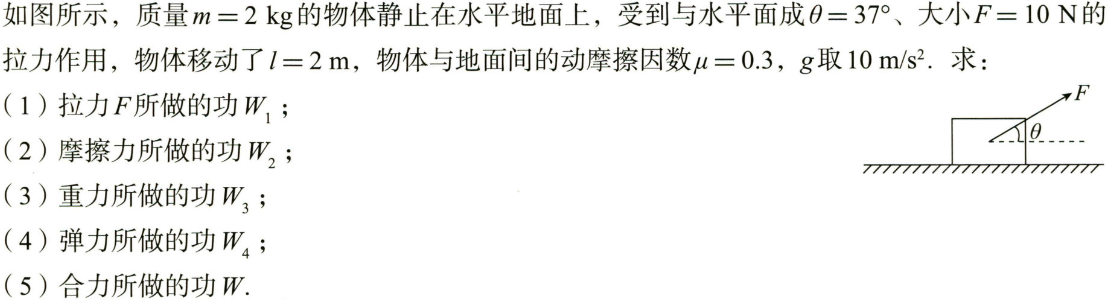
\includegraphics[width=0.9\textwidth]{pictures/1.png}

                  \vspace{1em}

                  \textbf{答案:}
                  \begin{enumerate}
                      \item[] $(1) \, W_{1} = 16 J \quad (2)\,W_{2} = -8.4J \quad (3)\,W_{3} = 0 \quad (4)\,W_{4} = 0 \quad (5)\,W = 7.6J$
                  \end{enumerate}

                  \textbf{解析:}
                  \begin{enumerate}[label=(\arabic*)]
                      \item $W_{1} = Fl\cos{\theta} = 10 \cross 2 \cross \frac{4}{5} = 16 J$
                      \item $N = mg - F\sin{\theta} = 14 N \quad f = - N \mu = -4.2N \quad W_{2} = fl = -4.2 \cross 2 = -8.4J$
                      \item $W_{3} = 0$
                      \item $W_{4} = 0$
                      \item $F = F\cos{\theta} + f = 10 \cross \frac{4}{5} - 4.2 = 3.8N \quad W = Fl = 3.8 \cross 2 = 7.6J$
                  \end{enumerate}

                  \vspace{2em}

                  \textbf{检测:}

                  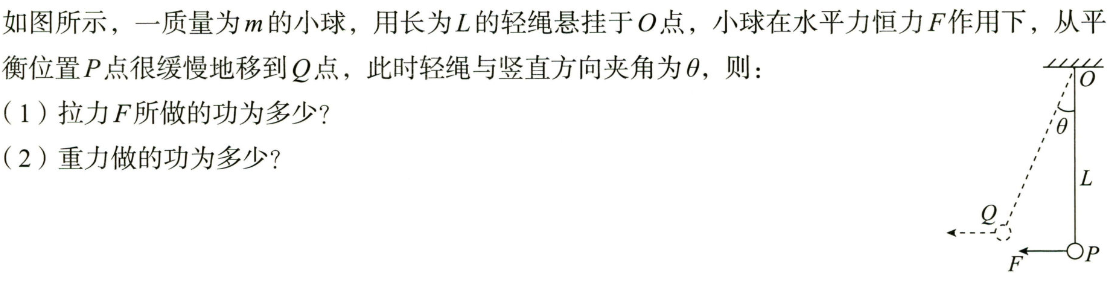
\includegraphics[width=0.9\textwidth]{pictures/2.png}

                  \vspace{1em}

                  \textbf{答案:}
                  \begin{enumerate}
                      \item[] $(1)\,W_{F} = FL\sin{\theta} \quad (2)\,W_{G} = -mgL(1-\cos{\theta})$
                  \end{enumerate}

                  \textbf{解析:}
                  \begin{enumerate}[label=(\arabic*)]
                      \item $W_{F} = F x_{F} = F L \sin{\theta} $
                      \item $W_{G} = -mg x_{G} = -mg(L - L \cos{\theta}) = -mgL(1-\cos{\theta})$
                  \end{enumerate}

                  \textbf{扩展:}
                  \begin{enumerate}[label=(\arabic*)]
                      \item 绳子拉力$T$所做的功$W_{T}$? $\lra W_{T} = 0$
                      \item 若受到空气阻力$f$大小不变,试问$W_{f}$? $\lra W_{f} = -f \cross 2\pi L \cross \frac{\theta}{2 \pi} = -fL\theta $
                  \end{enumerate}

                  \vspace{2em}

                  \textbf{检测:}

                  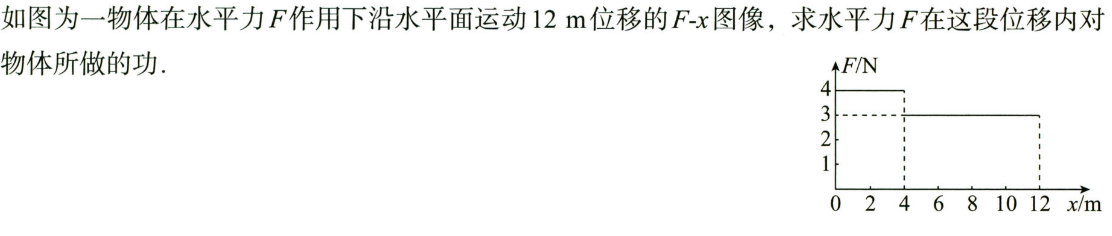
\includegraphics[width=0.9\textwidth]{pictures/3.png}

                  \vspace{1em}

                  \textbf{答案:}
                  \begin{enumerate}[label=(\arabic*)]
                      \item[] $W_{F} = 40J $
                  \end{enumerate}

                  \textbf{解析:}
                  \begin{enumerate}[label=(\arabic*)]
                      \item[] $W_{F} = 4 \cross 4 + 3 \cross 8 = 16 +24 = 40J $
                  \end{enumerate}

                  \textbf{扩展:}
                  \begin{enumerate}[label=(\arabic*)]
                      \item $0-4m\text{内},F = -4N \text{不变},W_{F}$? $\lra W_{F} = -4 \cross 4 + 3 \cross 8 = -16 + 24 = 8J$
                      \item 若$F = kx \hspace{0.5em} (k>0)$,试问当位移从$0$到$x_{0}$,整个过程$W_{F}$? $\lra W_{F} = \frac{1}{2} k x_{0}^{2}$
                      \item []

                            \begin{align*}
                                \triangle x     & = \dfrac{x_{0}}{n} \hspace{0.5em} (n \rightarrow \infty) \hspace{2em}
                                x_{i} = i \triangle x \hspace{0.5em}(i = 1,2,3 \cdots \infty)                                                                                                           \\
                                \triangle W_{i} & = F_{i} \triangle x = k x_{i} \triangle x  \hspace{2em} \sum_{i=1}^{n}\triangle W_{i} =
                                k(x_{1}+x_{2}+x_{3} \cdots x_{n} )\triangle x                                                                                                                           \\
                                W               & = k \triangle x (\triangle x + 2 \triangle x +3 \triangle x \cdots + n \triangle x) = k \triangle x \qty{ \dfrac{(\triangle x + n \triangle x)n}{2} } \\
                                W               & = \dfrac{k}{2} \qty{ n (\triangle x)^{2} + (n \triangle x)^{2}}  \hspace{2em} n\triangle x = x_{0}                                                    \\
                                W               & = \dfrac{k}{2} \qty{ x_{0} \triangle x + x_{0}^{2}}  \quad x_{0} \triangle x \text{相比} x_{0}^{2} \text{为小量舍去}                                         \\
                                W               & = \frac{1}{2} k x_{0}^{2}
                            \end{align*}
                  \end{enumerate}

                  \vspace{2em}

              \item[二、] 动能(Kinetic Energy)与动能定理
                  \begin{enumerate}
                      \item 动能定义:物体运动时所具备的能量(标量)$E_{k} = \frac{1}{2}mv^{2}$,单位\textbf{焦耳$J$}
                      \item 动能定理:合力对物体所做的功,等于物体动能的差$W_{total} = \triangle E_{k} = E_{kt} - E_{k0}$
                            $$
                                W_{total} = \va{F}_{total} \vdot \va{x} = W_{1} + W{2} \cdots W_{n}
                            $$

                            \begin{proof}
                                \begin{align*}
                                    2\va{a} \vdot \va{x}                                                    & = v_{t}^{2} - v_{0}^{2}                                                                \\
                                    2 \dfrac{\va{F}_{total}}{m} \vdot \va{x} = v_{t}^{2} - v_{0}^{2}  \quad & \lra  \quad \va{F}_{total} \vdot \va{x} = \frac{1}{2}mv_{t}^{2} -\frac{1}{2}mv_{0}^{2}
                                \end{align*}
                            \end{proof}

                      \item 理解:

                            初始状态$A\quad$ |$\lla$ $\quad$ 外部输入能量$W$($\pm J$) $\quad$ | $\quad \xlongequal{\quad\quad}$ 状态B
                            
                            \vspace{2em}

                            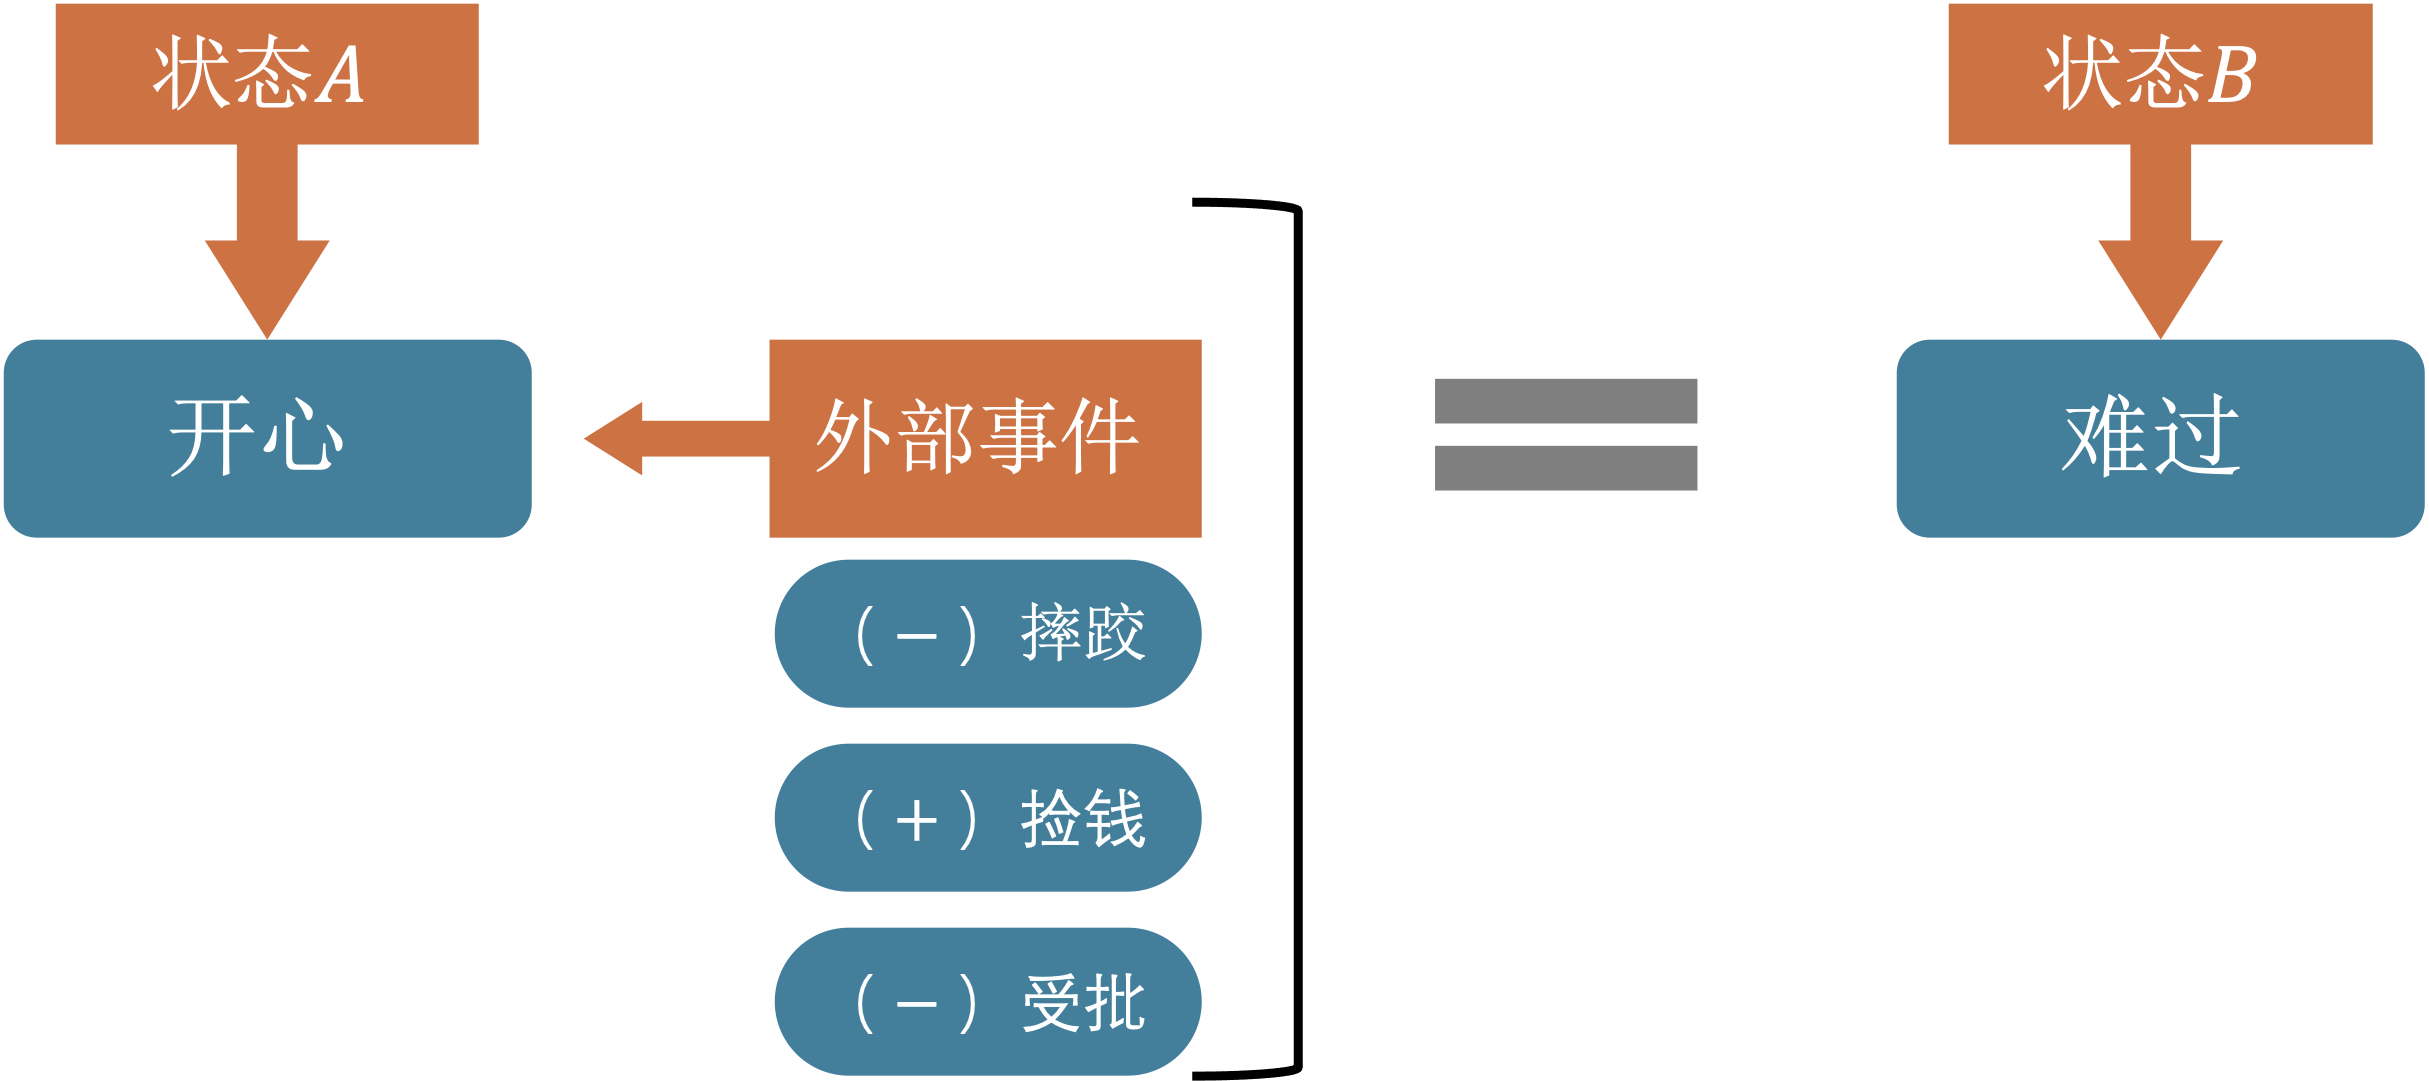
\includegraphics[width=0.7\textwidth]{pictures/4.png}

                  \end{enumerate}

          \end{enumerate}
\end{itemize}



\end{document}